\documentclass{ITaSconf}
\usepackage[utf8x]{inputenc}
\usepackage[russian]{babel}
\usepackage{url}

\usepackage{cancel}
\usepackage{graphicx}
\usepackage{amssymb}
\usepackage{amsmath}% http://ctan.org/pkg/amsmath
\usepackage{latexsym}
\usepackage{algorithm}
\usepackage{algorithmic}

\usepackage{subfig}

%\usepackage{algorithmic}
\newcommand{\x}{\mathbf{x}}
\newcommand{\h}{\mathbf{h}}
\newcommand{\w}{\mathbf{w}}
\newcommand{\W}{\mathbf{W}}
\newcommand{\y}{\mathbf{y}}
\newcommand{\X}{\mathbf{X}}
\newcommand{\Y}{\mathbf{Y}}
\newcommand{\fx}{\mathbf{f}}
\newcommand{\fs}{\mbox{f}}
\newcommand\argmin{\arg\min}

\newcommand\argmax{\arg\max}
\newcommand\headline{\hline}

\newcommand\sign{\mbox{sign}}

\title{Вероятностный подход для задачи предсказания биологической активности ядерных рецепторов}
\author{
	Володин Сергей \\
	\begin{affiliation}
		МФТИ
	\end{affiliation}\\
	\email{sergei.volodin@phystech.edu}
	\and
	Попова Мария \\
	\begin{affiliation}
		МФТИ
	\end{affiliation}\\
	\email{maria\_popova@phystech.edu}
}

\begin{document}
	\maketitle
	\begin{abstract}
Решается задача предсказания биологической активности молекул протеинов (лиганд) с рецепторами: по признакам лиганда необходимо оценить вероятность связывания этой молекулы с одним или несколькими клеточными рецепторами и построить бинарный классификатор. Экспертные знания в области биохимии и фармакологии дают основания предполагать, что факты связывания одних и тех же молекул с различными рецепторами не независимы. В данной работе предлагается модель, позволяющая строить предсказания сразу для группы рецепторов, учитывая их схожесть. Модель оценивает условные вероятности принадлежности классам. В работе проводится вычислительный эксперимент на реальных данных, в ходе которого предложенная модель сравнивается с независимыми моделями в терминах нескольких функционалов качества.
	\end{abstract}

\section{Введение}
Проблема предсказания биологической активности лигандов и рецепторов является актуальной задачей в области биохимии и фармакологии \cite{hornak, Myint2012, Myint2015, vinay2008, Zhengjun5ht1a, laurent2008}. Данная статья посвящена решению этой задачи методами машинного обучения.

Компьютерное моделирование взаимодействия молекул является распространенным методом предсказания биологической активности клеточных рецепторов \cite{vinay2008, hornak}. Однако такой способ требует знания точной структуры лиганд, которая не всегда известна. По этой причине развитие методов машинного обучения \cite{peter1998}, позволяющих делать предсказания на основании только числовых признаков лиганд, является актуальным.

Существует два основных подхода к решению описанной задачи. В рамках первого из них для каждого клеточного рецептора строятся независимые модели. Так, например в \cite{svm, Zhengjun5ht1a} применяется метод опорных векторов, в \cite{Myint2012, Myint2015}~--- нейронные сети, а в \cite{scott2006}~--- метод k ближайших соседей. Второй подход подразумевает построение одной модели для предсказания активности группы рецепторов. Такой подход позволяет строить более сложные модели, учитывающие информацию о схожести рецепторов \cite{laurent2008}. В \cite{popova1} проведен сравнительный анализ обоих подходов.

Таким образом, данная задача решается многими способами. Тем не менее, как показывает сопоставление результатов \cite{popova1}, лучшим оказывается второй подход, т.е. классификаторы, учитывающие при обучении все рецепторы сразу, а не независимо друг от друга. В данном случае это означает использование нескольких классификаторов и объеднение их в <<цепочку>> \cite{elena, weiweicc, jesse}. Как показывает практика, обучение нескольким задачам сразу дает существенный прирост в качестве конечного алгоритма по сравнению с рассмотрением этих задач по-отдельности \cite{weiwei2010, maxime2015, jesse}.

В данной работе предлагается усовершенствованный метод classifier chains \cite{jesse}~--- вероятностная модель последовательного вывода для предсказания биологической активности рецепторов \cite{enrique, weiwei2010}. Предложенный алгоритм относится ко второму подходу, то есть позволяет строить предсказания для группы рецепторов, а также допускает добавление новых без необходимости повторного обучения. Проведен вычислительный эксперимент на реальных данных, в котором набор независимых моделей сравнивался с моделью последовательного вывода. Построенные модели сравнивались по нескольким критериям качества.
\section{Постановка задачи классификации}
Задана выборка $\mathfrak{D}=\{(\x_i,\y_i)\}_{i\in \mathcal{L}}, \mathcal{L}=\{1,\dots, m\}$~--- $m$ пар объект-ответ. Каждый из объектов $\x_i\in \mathbb{R}^n$~--- вектор действительных чисел. Объект может принадлежать каждому из $l$, что представляется вектором ответов $\y_i\in \{0,1,\Box\}^l$, $1$ означает принадлежность классу, а $\Box$ означает пропуск в данных. Выборка разбита на обучающую и контрольную: $\mathfrak{D}=\mathfrak{L}\sqcup\mathfrak{T}$

%$\X=\mathbb{R}^n$~--- пространство независимых переменных (объектов), $\Y=\{0,1\}^l$~--- пространство всех ответов.

Определяются $\X, \Y$~--- случайные величины.
% на пространстве $\X\times\Y$
Считается, что между классами есть зависимости:
$$P(\Y|\X)\neq \prod_{j=1}^l P(y_j|\X)$$
%Вводится предположение, что условное распределение $P(\X|\Y)$ принадлежит семейству экспоненциальных распределений.

%Рассмотрим \cite{weiwei2010} величину $P(\y|\x)=P(y_1|\x)\cdot\prod_{i=2}^lP(y_i|y_1,...,y_{i-1},\x)$~--- по свойству вероятности. Из этой формулы следует, что вероятность $P(\y|\x)$ можно найти как произведение вероятностей, причем $i$-я обусловлена по значению $i-1,...,1$ признаков.

%Моделью классификации назовем функцию $\fx\colon \W\times\X\to [0,1]^M$ вида $\fx(\w,\x)=\fx_l(\fx_{l-1}(...\fx_1(\w_1,\x_1)...))$, где $\w=(\w_1,...,\w_l)$~--- вектор параметров модели, $\W=\W_1\times\dots\times\W_l$~--- множество параметров. $\fx_1\colon\X\to\X\times[0,1]$, ..., $\fx_k\colon \X\times [0,1]^{k-1}\to\X\times [0,1]^k$. Компоненты $\fx$~--- апостериорные вероятности принадлежности объекта к соответствующему классу:

Моделью классификации называется функция
$$\fs\colon \W\times\X\times\Y\to [0,1],$$
где $\W$~--- множество параметров, $\w\in\W$~--- вектор параметров модели. Значение $\fs$~--- апостериорая вероятность ответов $\y$ при фиксированном $\x$:
$$\fs(\w,\x,\y)=P(\Y=\y|\X=\x;\w)$$

%Из сделанных предположений относительно параметров распределения следует, что $P(y_j=1|x)$

Функция потерь для значения параметра $\w$ и подвыборки $\mathcal{Z}$ определяется через функцию правдоподобия модельного распределения:
$$Q(\fs|\w, \mathcal{Z})=-\sum_{(\x,\y)\in\mathcal{Z}}\log \fs(\w,\x,\y)P(\X=\x)$$

%

Требуется найти вектор параметров $\w^*\in\W$, минимизирующий $Q$ на обучающей выборке $\mathfrak{L}$:
	$$\w^*=\argmin_{\w\in\W}Q(\fs|\w,\mathfrak{L})$$

Для вывода бинарного классификатора из вероятностной модели $P(\y|\x)$ вводится функция потерь, т.е. штраф за ответ $\y$ при правильном ответе $\y'\in\Y$:
$$L\colon Y\times Y\to \mathbb{R}$$

Бинарный классификатор $\h\colon\X\to\Y$ получается \cite{weiwei2010} при помощи Байесовского решающего правила:
$$\h(\x)=\argmin\limits_{\y\in\Y}\mathbb{E}_{\Y|\X}L(\Y,\y)$$

В качестве дополнительного критерия качества модели используются значения Subset Loss для векторов ответов, а также значения Hamming Loss и других метрик для каждого класса $j$ на контрольной выборке $\mathfrak{T}$ при 5 различных разбиениях.

%В качестве дополнительного критерия качества модели используются значения функционала AUC для каждого класса $j$ на контрольной выборке $\mathfrak{T}$ при 5 различных разбиениях. %:
%$$\mbox{AUC}_j(f_j,\w_j,\mathfrak{T})=\frac{1}{g_j(|\mathfrak{T}|-g_j)}\sum_{(\x,\y)\in\mathfrak{L}}\sum_{(\hat{\x},\hat{\y})\in\mathfrak{L}}[y_j<\hat{y}_j][f_j(\w_j,\x)<f_j(\w_j,\hat{\x})],$$
%где $g_j$~--- количество объектов в $\mathfrak{T}$ с $y_j=1$.

Поскольку выборка содержит пропуски, разбиения должны быть построены таким образом, чтобы в каждой подвыборке было достаточное количество объектов с известным значением каждого признака.

\section{Описание алгоритма}
Таким образом, задача предсказания разбивается на два этапа:
\begin{enumerate}
\item Поиск параметра модели $\w$ максимизацией правдоподобия выборки на семействе распределений $P(\y|\x;\w)$. В результате решения задачи получается модель $P_{\w^*}(\y|\x)$ как функция двух переменных
\item Поиск оптимального бинарного классификатора $h\colon \X\to\Y$, использующего найденное распределение $P(\y|\x)$. Конкретная функция получается применением Байесовского решающего правила для каждого $\x$, подлежащего классификации. Конкретный классификатор зависит от выбранной функции потерь $L$.
\end{enumerate}

\section{Часть 1. Предлагаемый вид модели}
Решим первую часть поставленной задачи, используя метод, описанный в \cite{weiwei2010}.

Рассмотрим искомую величину $$P(\y|\x)$$.

Докажем равенство $$P(\y|\x)=P(y_1|\x)\prod_{i=2}^lP(y_i|y_1,...,y_{i-1}, \x)$$

Рассмотрим величину $$P(y_i|y_1,...,y_{i-1},\x)=\frac{P(y_1,...,y_i,\x)}{P(y_1,...,y_{i-1},\x)}$$

Подставим их в произведение, получим телескопическое произведение: $$P(y_1|\x)\prod_{i=2}^lP(y_i|y_1,...,y_{i-1}, \x)=$$
$$=\frac{\cancel{P(y_1,\x)}}{P(\x)}\frac{\cancel{P(y_1,y_2,\x)}}{\cancel{P(y_1,\x)}}\cdot...\cdot\frac{P(y_1,...,y_l,\x)}{\cancel{P(y_1,...,y_{l-1},\x)}}=P(\y|\x)\,\blacksquare$$

Таким образом, для моделирования вероятности $P(\y|\x)$ можно использовать условные вероятности классов $$P(y_1|\x),\,P(y_2|y_1,\x)...,\,P(y_l|y_1,...,y_{l-1},\x)$$

Каждую из $l$ этих вероятностей будем оценивать при помощи логистической регрессии.

Обозначим $$(x)_{y}=\begin{cases}
x, & y = 1\\
1 - x & y = 0
\end{cases}$$

Обозначим $$g_i(y_1,...,y_{i-1},\x)=P(y_i=1|y_1,...,y_{i-1},\x)$$

Получаем выражение вероятности $P(\y|\x)$ через функции $g_i$: $$P(\y|\x)=P(y_1|\x)\prod\limits_{i=2}^lP(y_i|y_1,...,y_{i-1},\x)=\prod\limits_{i=1}^l(g_i(y_1,...,y_{i-1},\x))_{y_i}$$


Вероятности $$P(y_i=1|y_1,...,y_{i-1},\x)=g_i(y_1,...,y_{i-1},\x)$$
предсказываются при помощи логистической регрессии, т.е.
$$g_i(y_1,...,y_{i-1},\x)=\sigma(\w_i^T||y_1...y_{i-1}\x^T||^T+w^0_i)$$ где $$\sigma(x)=\frac{1}{1+e^{-x}}$$

Получаем семейство моделей $$P(\y|\x)=(\sigma(\w_1^T\x+w^0_1))_{y_1}\prod\limits_{i=2}^l(\sigma(\w_i^T||y_1...y_{i-1}\x^T||^T+w^0_i))_{y_i}$$

Таким образом, общая задача оптимизации $\w^*$ распадается на $l$ независимых оптимизационных задач максимизации правдоподобия, т.е. на обучение $l$ логистических регрессий. $i$-я логистическая регрессия принимает в качестве признаков $\x$, а также ответы $y_1,...,y_{i-1}$

Данный алгоритм называется PCC (Probabilistic Classifier Chain) \cite{weiwei2010}

\section{Часть 2. Бинарный классификатор}
Решим вторую часть задачи, т.е. построим бинарный классификатор по известному распределению $P(\y|\x)$, выбирая некоторую функцию потерь (см. \cite{weiwei2010}).

При фиксированной функции потерь $L$ и объекте $\x\in\X$ оптимальное предсказание $\h(\x)\in\Y$ в соответствии с Байесовским решающим правилом имеет вид \cite{weiwei2010}:
$$\h(\x)=\argmin\limits_{\y\in\Y}\mathbb{E}_{\Y|\X}L(\Y,\y)$$

%Покажем, как получить из вероятности $P(\y|\x)$ вероятности классов, а также как построить бинарный классификатор, выбирая некоторую функцию потерь (см. \cite{weiwei2010}).

В качестве примеров рассмотрим следующие функции потерь $L(\y,\y')$ и приведем полученный алгоритм $h(\x)$ \cite{weiwei2010}:

\begin{enumerate}
\item Hamming Loss. Получаем $h_i(\x)=\sign(P(y_i=1|\x)-\frac{1}{2})$
\item Subset 0/1 Loss. Получаем $h(\x)=\argmax_{y\in Y}P(\y|\x)$
\item Rank Loss. Получаем $f_i(\x)=P(y_i=1|\x)$
\end{enumerate}

Используемая вероятность $P(y_i=1|\x)$ может быть получена из известного распределения $P(\y|\x)$ по формуле полной вероятности:
$$P(y_i=1|\x)=\sum\limits_{y\in \{0,1\}^l}[y_i=1]P(\y|\x)$$

Таким образом, искомые вероятности выражаются через известное распределение $P(\y|\x)$.

%{\em Описать, как решается проблема с пропусками при обучении и придумать нормальный алгоритм (классификация уже имеющимися звеньями). Описать, как производить разбиение. Описать, как выбирать порог логистической регрессии $\frac{\lambda_+}{\lambda_-}$ по точке на ROC-кривой.}
\section{Часть 3. Работа с пропусками}
Приведенный выше алгоритм PCC построения $P(\y|\x)$ по имеющейся обучающей выборке неприменим для выборок, для которых в ответах могут содержаться пропуски: $y_i\in\{0,1,\Box\}$. Эта проблема решается следующим образом:
\begin{enumerate}
\item Логистические регрессии $1,...,l$ обучаются последовательно
\item Для обучения $i$-й логистической регрессии берутся объекты с известным значением признака $y_i$
\item Предыдущие неизвестные значения признаков $y_1,..,y_{i-1}$ предсказываются частично уже построенным PCC для классов $1,...,{i-1}$.
\end{enumerate}

\subsection{Алгоритмы}
\begin{algorithm}[H]
	\caption{Обучение PCC для выборок без пропусков}
	\label{PCCLearn}
	\begin{algorithmic}[1]
		\REQUIRE Обучающая выборка $\mathfrak{L}=\{(\x_i,\y_i)\}_{i\in L}$
		\ENSURE Векторы $\w_i\in\mathbb{R}^{n+i-1},\,i\in\overline{1,l}$
		
		\STATE {$u_j\leftarrow$ $j$-й столбец матрицы $y_{ij}$, $j\in\overline{1,l}$}
		\FOR {$i = 1, \dots, l$}
		\STATE {$X^i\leftarrow ||X y_1 ... y_{i-1}||^\Box$. Эта матрица имеет строки $X^i_j$}
		\STATE {$\w_i=\argmax{\prod\limits_{j\in L}}(\sigma(\w_i^TX^i_j))_{y_{ij}} $~--- обучение логистической регрессии}
		\ENDFOR
	\RETURN $\w_1,...,\w_l$
	\end{algorithmic}
\end{algorithm}
\begin{algorithm}[H]
	\caption{Предсказание вероятности $P(\y|\x)$ для пары объект-ответ}
	\label{PCCPredictSubset}
	\begin{algorithmic}[1]
		\REQUIRE Объект $\x\in \mathbb{R}^n$, векторы $\w_i$, пороги $w^0_i$, вектор $\y\in\{0,1\}^m$
		\ENSURE Условная вероятность $P(\y|\x)\in[0,1]$
		
		\STATE {$P\leftarrow 1$}
		\FOR {$i = 1, \dots, l$}
		\STATE {$\x'\leftarrow ||\x^T y_1 ... y_{i-1}||^{\Box T}$}
		\STATE {$P\leftarrow P \cdot (\sigma(\w_i^T\x'+w^0_i))_{y_i}$}
		\ENDFOR
	\RETURN P
	\end{algorithmic}
\end{algorithm}

\section{Вычислительный эксперимент}

%\section{Базовый вычислительный эксперимент}
Целью эксперимента является получение характеристик предложенного алгоритма и сравнение результатов с базовым алгоритмом. Также в ходе эксперимента находятся значения гиперпараметров исходя из оптимизации функций ошибок.

Базовый алгоритм использует подход Binary Relevance \cite{weiwei2010}, в котором зависимости между классами не учитываются. Таким образом, алгоритм представляет собой $l$ независимых логистических регрессий, по одному классификатору для каждого класса. Предлагаемый алгоритм, PCC, учитывает зависимости между классами.

Для решения второй части задачи в предлагаемом алгоритме рассматриваются следующие функции потерь:
\begin{enumerate}
	\item Subset 0/1 loss: $L(\y, \y')=[\y\neq \y']$
	\item Hamming loss: $L(\y,\y')=\sum\limits_{i=1}^l[y_i\neq y'_i]$
	\item Функционал $L(\y,\y')=q\left(\sum\limits_{i=1}^l[y_i\neq y'_i]\right)$, где $q(t)$ задана в натуральных точках $t\in\overline{0,l}$ и подлежит оптимизации.
\end{enumerate}

Для полученных результатов бинарных классификаторов также сравниваются значения Precision, Recall, Hamming loss и AUC для каждого класса, а также Hamming Loss и Subset Loss вцелом. Для оценки стандартного отклонения используется $5$-fold разбиение. Эксперимент проведен на модельных и реальных данных.
% и энтропийный критерий информативности $$I(p, n, l, P)=h\left(\frac{P}{l}\right)-\frac{p+n}{l}h\left(\frac{p}{p+n}\right)-\frac{l-p-n}{l}h\left(\frac{P-p}{l-p-n}\right),$$ $$h(q)=-q\log_2q-(1-q)\log_2(1-q)$$

\subsection{Модельные данные}
Используется следующая вероятностная модель для генерации выборки:

Выборка $\mathfrak{D}=\{(x_i,\y_i)\}_{i\in \mathcal{L}}, \mathcal{L}=\{1,\dots, m\}$~--- $m$ пар объект-ответ. Каждый из объектов $x_i\in [-1.5,1.5]$~--- действительное число. Объект может принадлежать каждому из $l=3$ классов, что представляется вектором ответов $\y_i\in \{0,1\}^l$, $1$ означает принадлежность классу. В модельных данных пропуски в ответах отсутствуют.

Вероятность принадлежности объекта $x$ к классам $\y\in\{0,1\}^3$ $P(\y|x)$ задается по формуле \cite{weiwei2010}:
$$P(y_1,y_2,y_3|x)=(f_1(x))_{y_1}(f_2(x, y_1))_{y_2}(f_3(x, y_1, y_2))_{y_3},$$
где $f_1,f_2,f_3$ заданы следующим образом:
$$
\begin{array}{rl}
f_1(x)= & \sigma(x)\\
f_2(x, y_1) =& \sigma(x-2y_1+1)\\
f_3(x, y_1, y_2) =& \sigma(x+12y_1-2y_2-11)\\
\end{array}
$$

Выборка содержит $500$ объектов. Генерация производится следующим образом:
\begin{enumerate}
	\item Выбирается $x\sim u[-1.5,1.5]$~--- из равномерного распределения
	\item Выбирается $\y$ для данного $x$ в соответствии с формулой.
\end{enumerate}

% Выборка разбита на обучающую и контрольную: $\mathfrak{D}=\mathfrak{L}\sqcup\mathfrak{T}$

Полученные плотности $P(\y|x)$ изображены на графике \ref{fg:ModelData}.

Для сравнения алгоритмов использовались следующие метрики: $\mbox{AUC}_i$~--- AUC для каждого класса, $\mbox{H}_i$~--- Hamming Loss для каждого класса, $\mbox{P}_i$~--- Precision, $\mbox{R}_i$~--- Recall, $\mbox{S}$~--- Subset Loss, $\mbox{H}$~--- общий Hamming Loss.

Для контроля переобучения используется 5-fold кросс-валидация.

В качестве функций потерь для PCC использовались следующие: H (Hamming Loss), S (Subset Loss), а также M~--- функция вида
$$L(\y,\y')=q\left(\sum\limits_{i=1}^l[y_i\neq y'_i]\right),$$

Функция $q$ определена в точках $\overline{0,l}=\overline{0,3}$. Проведена оптимизация $q$ по различным метрикам итогового алгоритма. Значения $q$ в точках $(0,1,2,3)$ имеют вид $(0,a_1,a_2,10)$, где $a_1,a_2$ подлежат перебору.

Оптимальная функция $q$ зависит от метрики и класса, для которого вычисляется данная метрика.

Показано, что для оптимизации Subset Loss $a_1=10,a_2=10$, а для оптимизации суммарного Hamming Loss $a_1=2, a_2=5$. В качестве $q_M$ взята последняя.

Результаты представлены в таблице \ref{fg:ModelData}. Наблюдается серьезное улучшение в Subset Loss для PCC (S). Остальные изменения в пределах погрешности.

График \ref{fg:ModelData} показывает зависимость функции ошибки Subset Loss на обучающей и контрольной выборке от мощности обучающей выборки. Видно, что при $|\mathfrak{L}|<100$ ошибка на контроле сильно больше ошибки на обучении, т.е. возникает переобучение. При $|\mathfrak{L}|\gtrsim 150$ этот эффект уходит, и ошибки становятся примерно равны. На графике \ref{t:modelData} представлена зависимость Subset Loss на обучении и контроле от коэффициента регуляризации $C$. В силу тривиальности выборки Subset Loss слабо зависит от этого коэффициента.

Графики \ref{t:modelData} показывают время выполнения алгоритмов обучения и предсказания в зависимости от размера выборки. Оценим время предсказания как $2^{2l}\cdot n$, где $n$~--- размер выборки, $l$~--- количество классов. По $n$ эта зависимость линейна.

\subsection{Реальные данные}
Эксперимент проведен на реальных данных, имеющих двойное происхождение. Объектами являются лиганды, их признаки $\x_i$ смоделированы при помощи специальной программы. Ответы $\y_i=(y_{i1},...,y_{il})$ являются результатами биохимических экспериментов, показывающих, связывается ли данный лиганд с рецептором $j$. Пропуск в ответах означает, что эксперимент либо не был проведен, либо не позволяет с достаточной уверенностью говорить о каком-либо результате. Каждый объект имеет $165$ признаков. Признаки являются химическими параметрами молекулы. В выборке содержится $8513$ объектов, количество объектов с измеренным ответом $j$ составляет около половины. В таблице \ref{t:dataDescr} указано точное распределение ответов по классам. График \ref{fg:realFeatures} показывает распределение объектов по значениям всех $165$ признаков. Видно, что большинство распределений унимодальные.

График \ref{fg:VIF} показывает распределение признаков по значению $R^2=1-\frac{1}{\mbox{VIF}}$. Видно, что данные обладают высокой мультиколлинеарностью (большинство признаков имеют $R^2$, близкий к 1)

На графиках (\ref{fg:BR}) показаны ROC-кривые классов для одного из разбиений, построенные по предсказаниям Binary Relevance, а также значение функционала AUC. В таблице \ref{t:methodCmp} приведено сравнение метода Binary Relevance с результатами из \cite{qsar}, для получения которых использовались те же данные, что и в данной работе. Сравнение результатов показывает, что логистическая регрессия уступает в качестве классификации методу Random Forest. Для некоторых рецепторов эта разница значительна.

Для определения эффективности методов вычисляются значения метрик Hamming Loss, Subset Loss, Precision, Recall для каждого из разбиений $\mathfrak{D}=\mathfrak{L}\sqcup\mathfrak{T}$ на тестовую и контрольную выборку. Вычисляются средние значения и стандартные отклонения. Разбиения выполнены по методу Shuffle Split с размером тестовой выборки $0.1$ и количеством разбиений $5$ из-за разреженности данных. Используются функции потерь для PCC, аналогичные таковым для модельных данных. В эксперименте использованы только данные по рецепторам NR-AhR, NR-AR-LBD, NR-Aromatase. Использованы только объекты со всеми тремя известными ответами.

%. Вычисляется среднее значение AUC, а также стандартное отклонение.

%['NR-AhR' 'NR-AR-LBD' 'NR-AR' 'SR-MMP' 'NR-ER' 'SR-HSE' 'SR-p53' 'NR-PPAR-gamma' 'SR-ARE' 'NR-Aromatase' 'SR-ATAD5' 'NR-ER-LBD']

Результаты сравнения PCC и BR представлены в таблице \ref{t:realData}. Как и для модельных данных, заметно существенное улучшения Subset Loss для PCC (S). Также имеется незначительное улучшение Hamming Loss (H) для класса 2 (NR-AR-LBD).

\section{Заключение}

В работе применен алгоритм Probabilistic Classifier Chains для решения задачи предсказания взаимодействия рецепторов и лигандов. Алгоритм сравнивается с базовым алгоритмом, не учитывающим зависимости между классами. Вычислительный эксперимент показал, что как для модельных, так и для реальных данных PCC позволяет существенно улучшить показатели Subset Loss, т.е. качество предсказания всего вектора. При использовании Hamming Loss результаты сходны с результатами независимого классификатора. Предложена функция потерь для алгоритма PCC, позволяющая незначительно улучшить показатели Hamming Loss для отдельных классов.

\begin{figure}[h]
	\subfloat[Гистограмма $R^2$ для реальных данных]{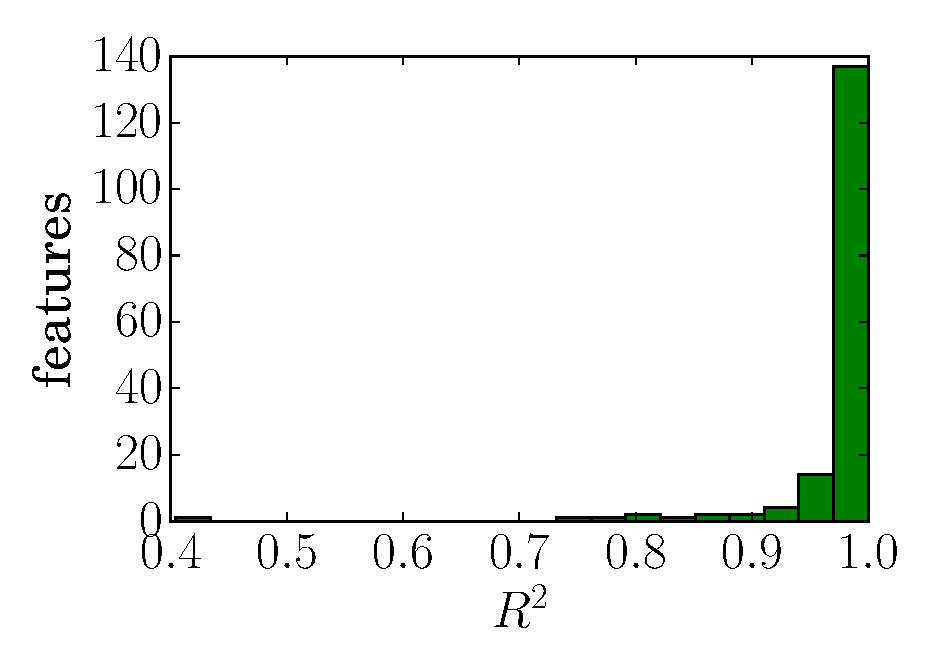
\includegraphics[width=0.5\textwidth]{RealDataVIF}}
	\caption{Реальные данные}
	\label{fg:VIF}
\end{figure}


\begin{figure}[h]
	\subfloat[Плотность модельных данных]{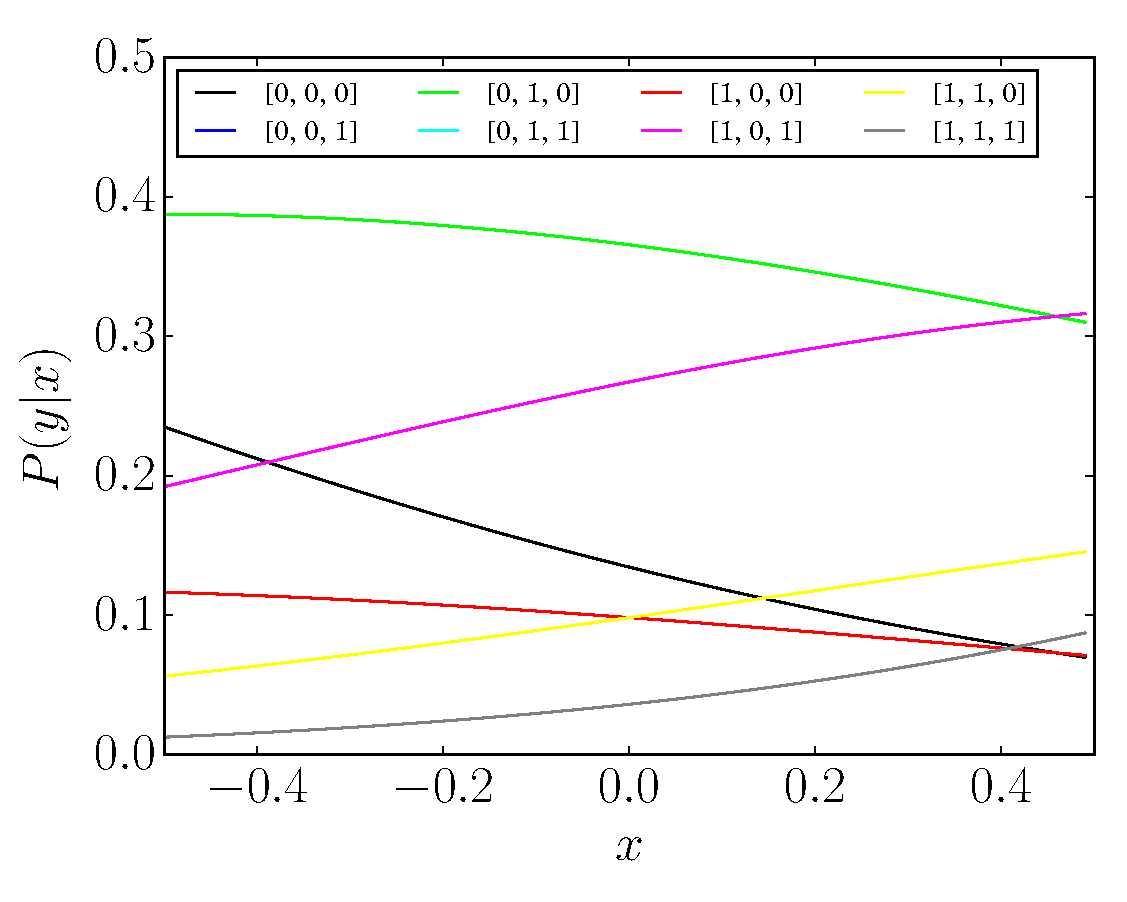
\includegraphics[width=0.5\textwidth]{ModelData}}
	\subfloat[Зависимость ошибки на обучении и контроле от размера обучающей выборки]{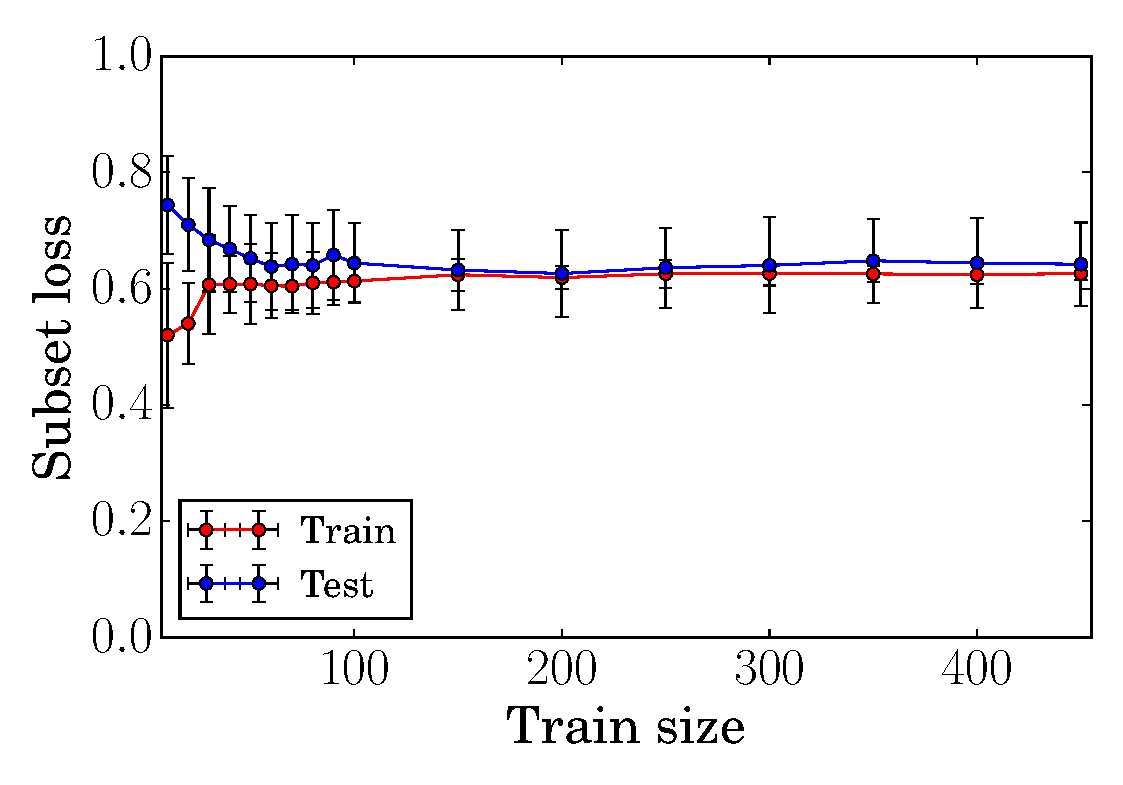
\includegraphics[width=0.5\textwidth]{ModelDataTrainSize}}\\
	\subfloat[Зависимость ошибки на обучении и контроле от коэффициента регуляризации]{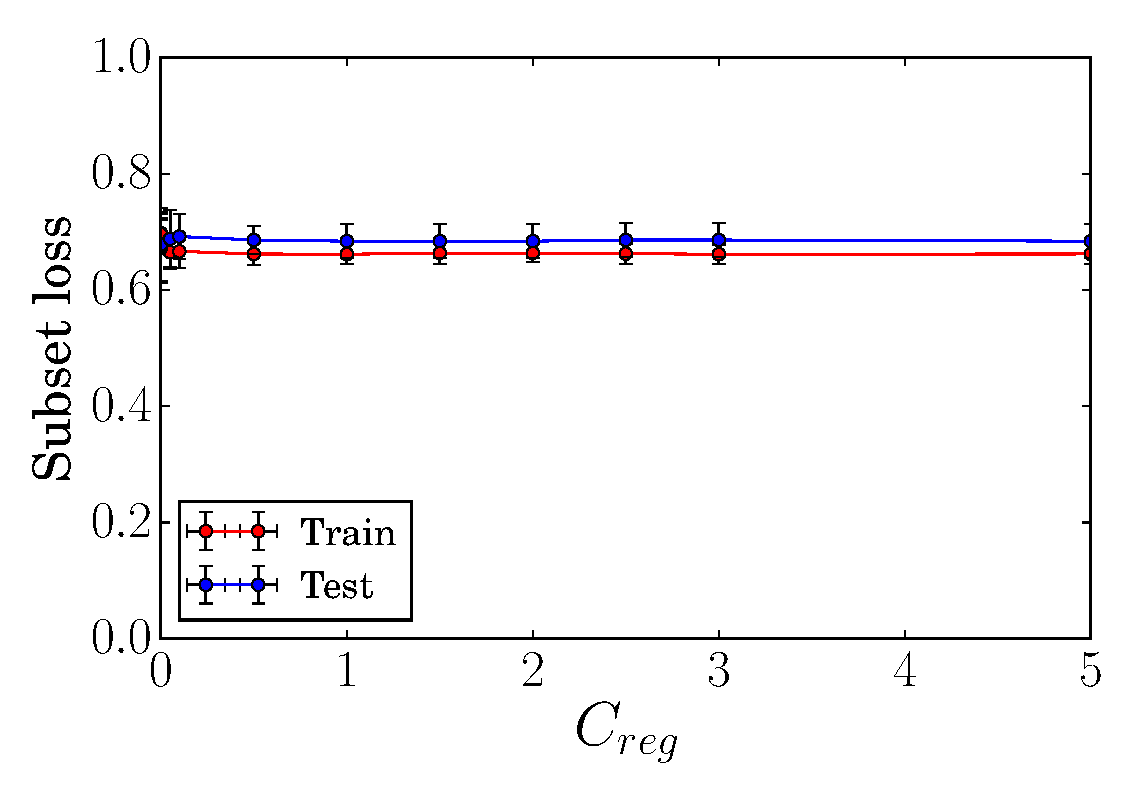
\includegraphics[width=0.5\textwidth]{ModelDataReg}}
	\subfloat[Время обучения в зависимости от размера выборки]{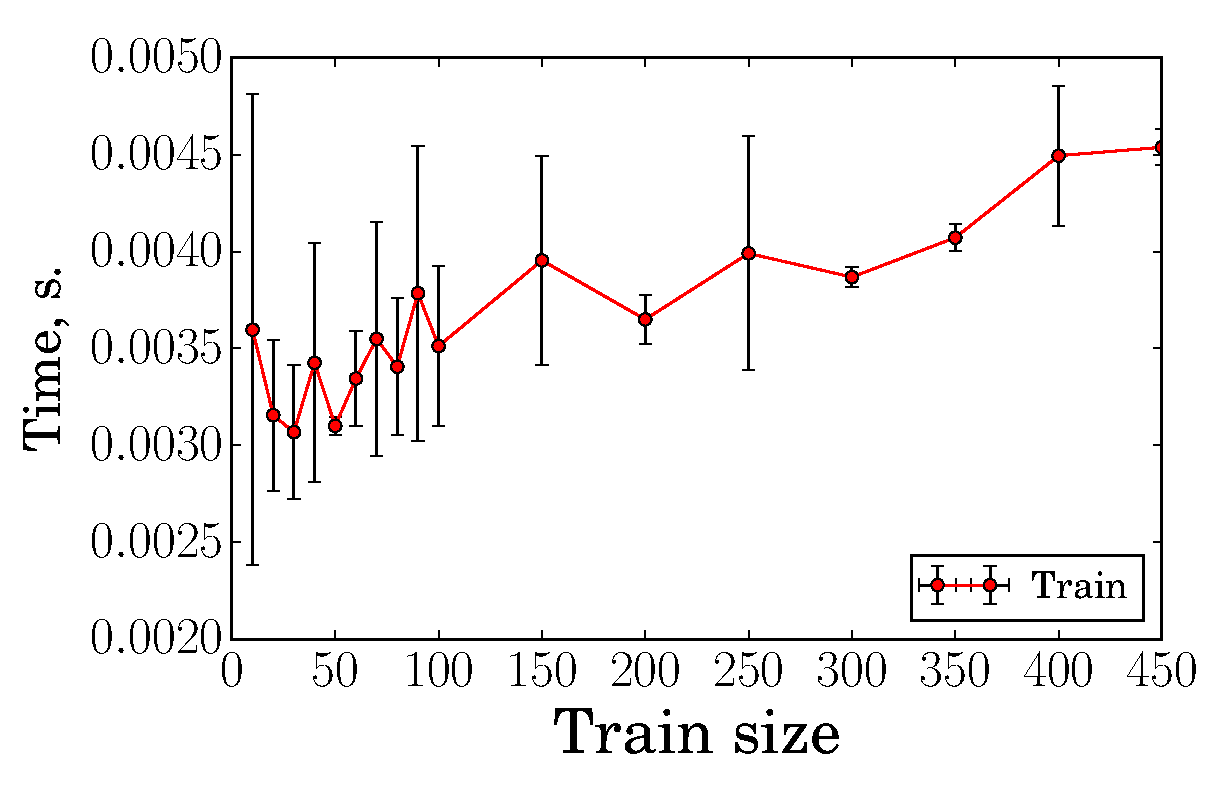
\includegraphics[width=0.5\textwidth]{ModelDataTimingTrain}}\\
	\subfloat[Время предсказания в зависимости от размера выборки]{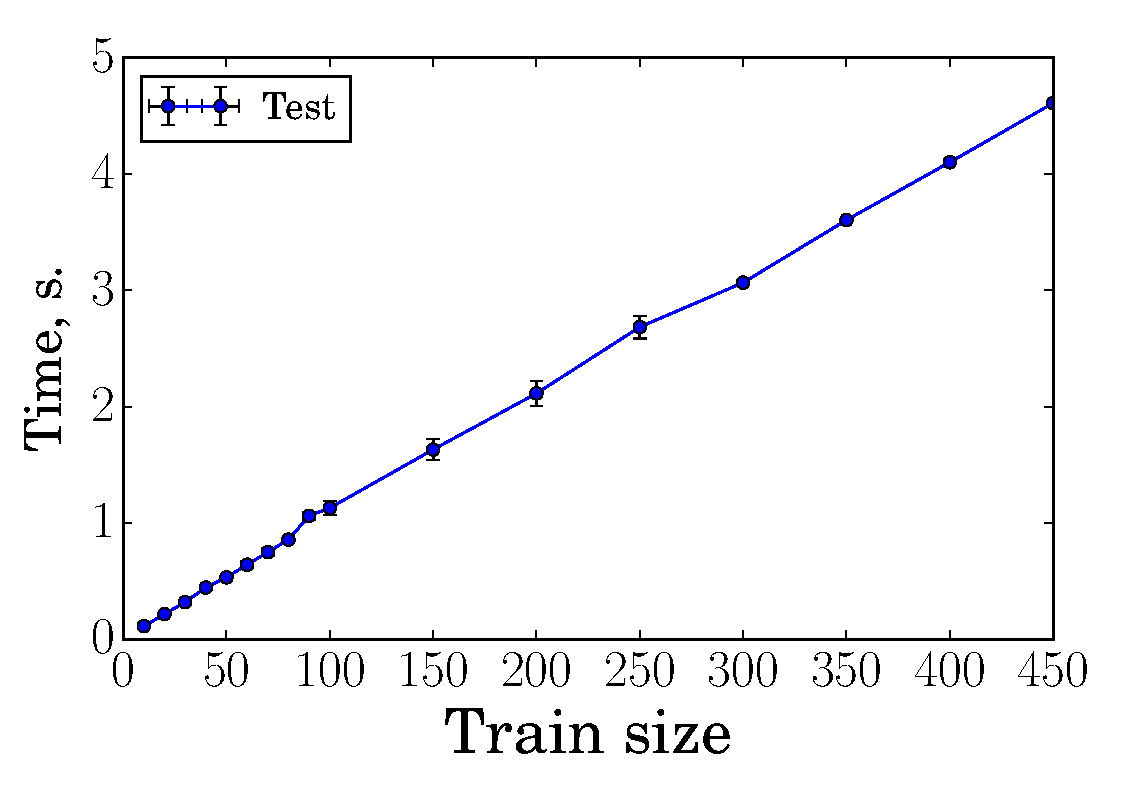
\includegraphics[width=0.5\textwidth]{ModelDataTimingTest}}
	\caption{Модельные данные}
	\label{fg:ModelData}
\end{figure}

\begin{figure*}[p]
	\subfloat[Распределение объектов по значениям признаков для реальных данных]{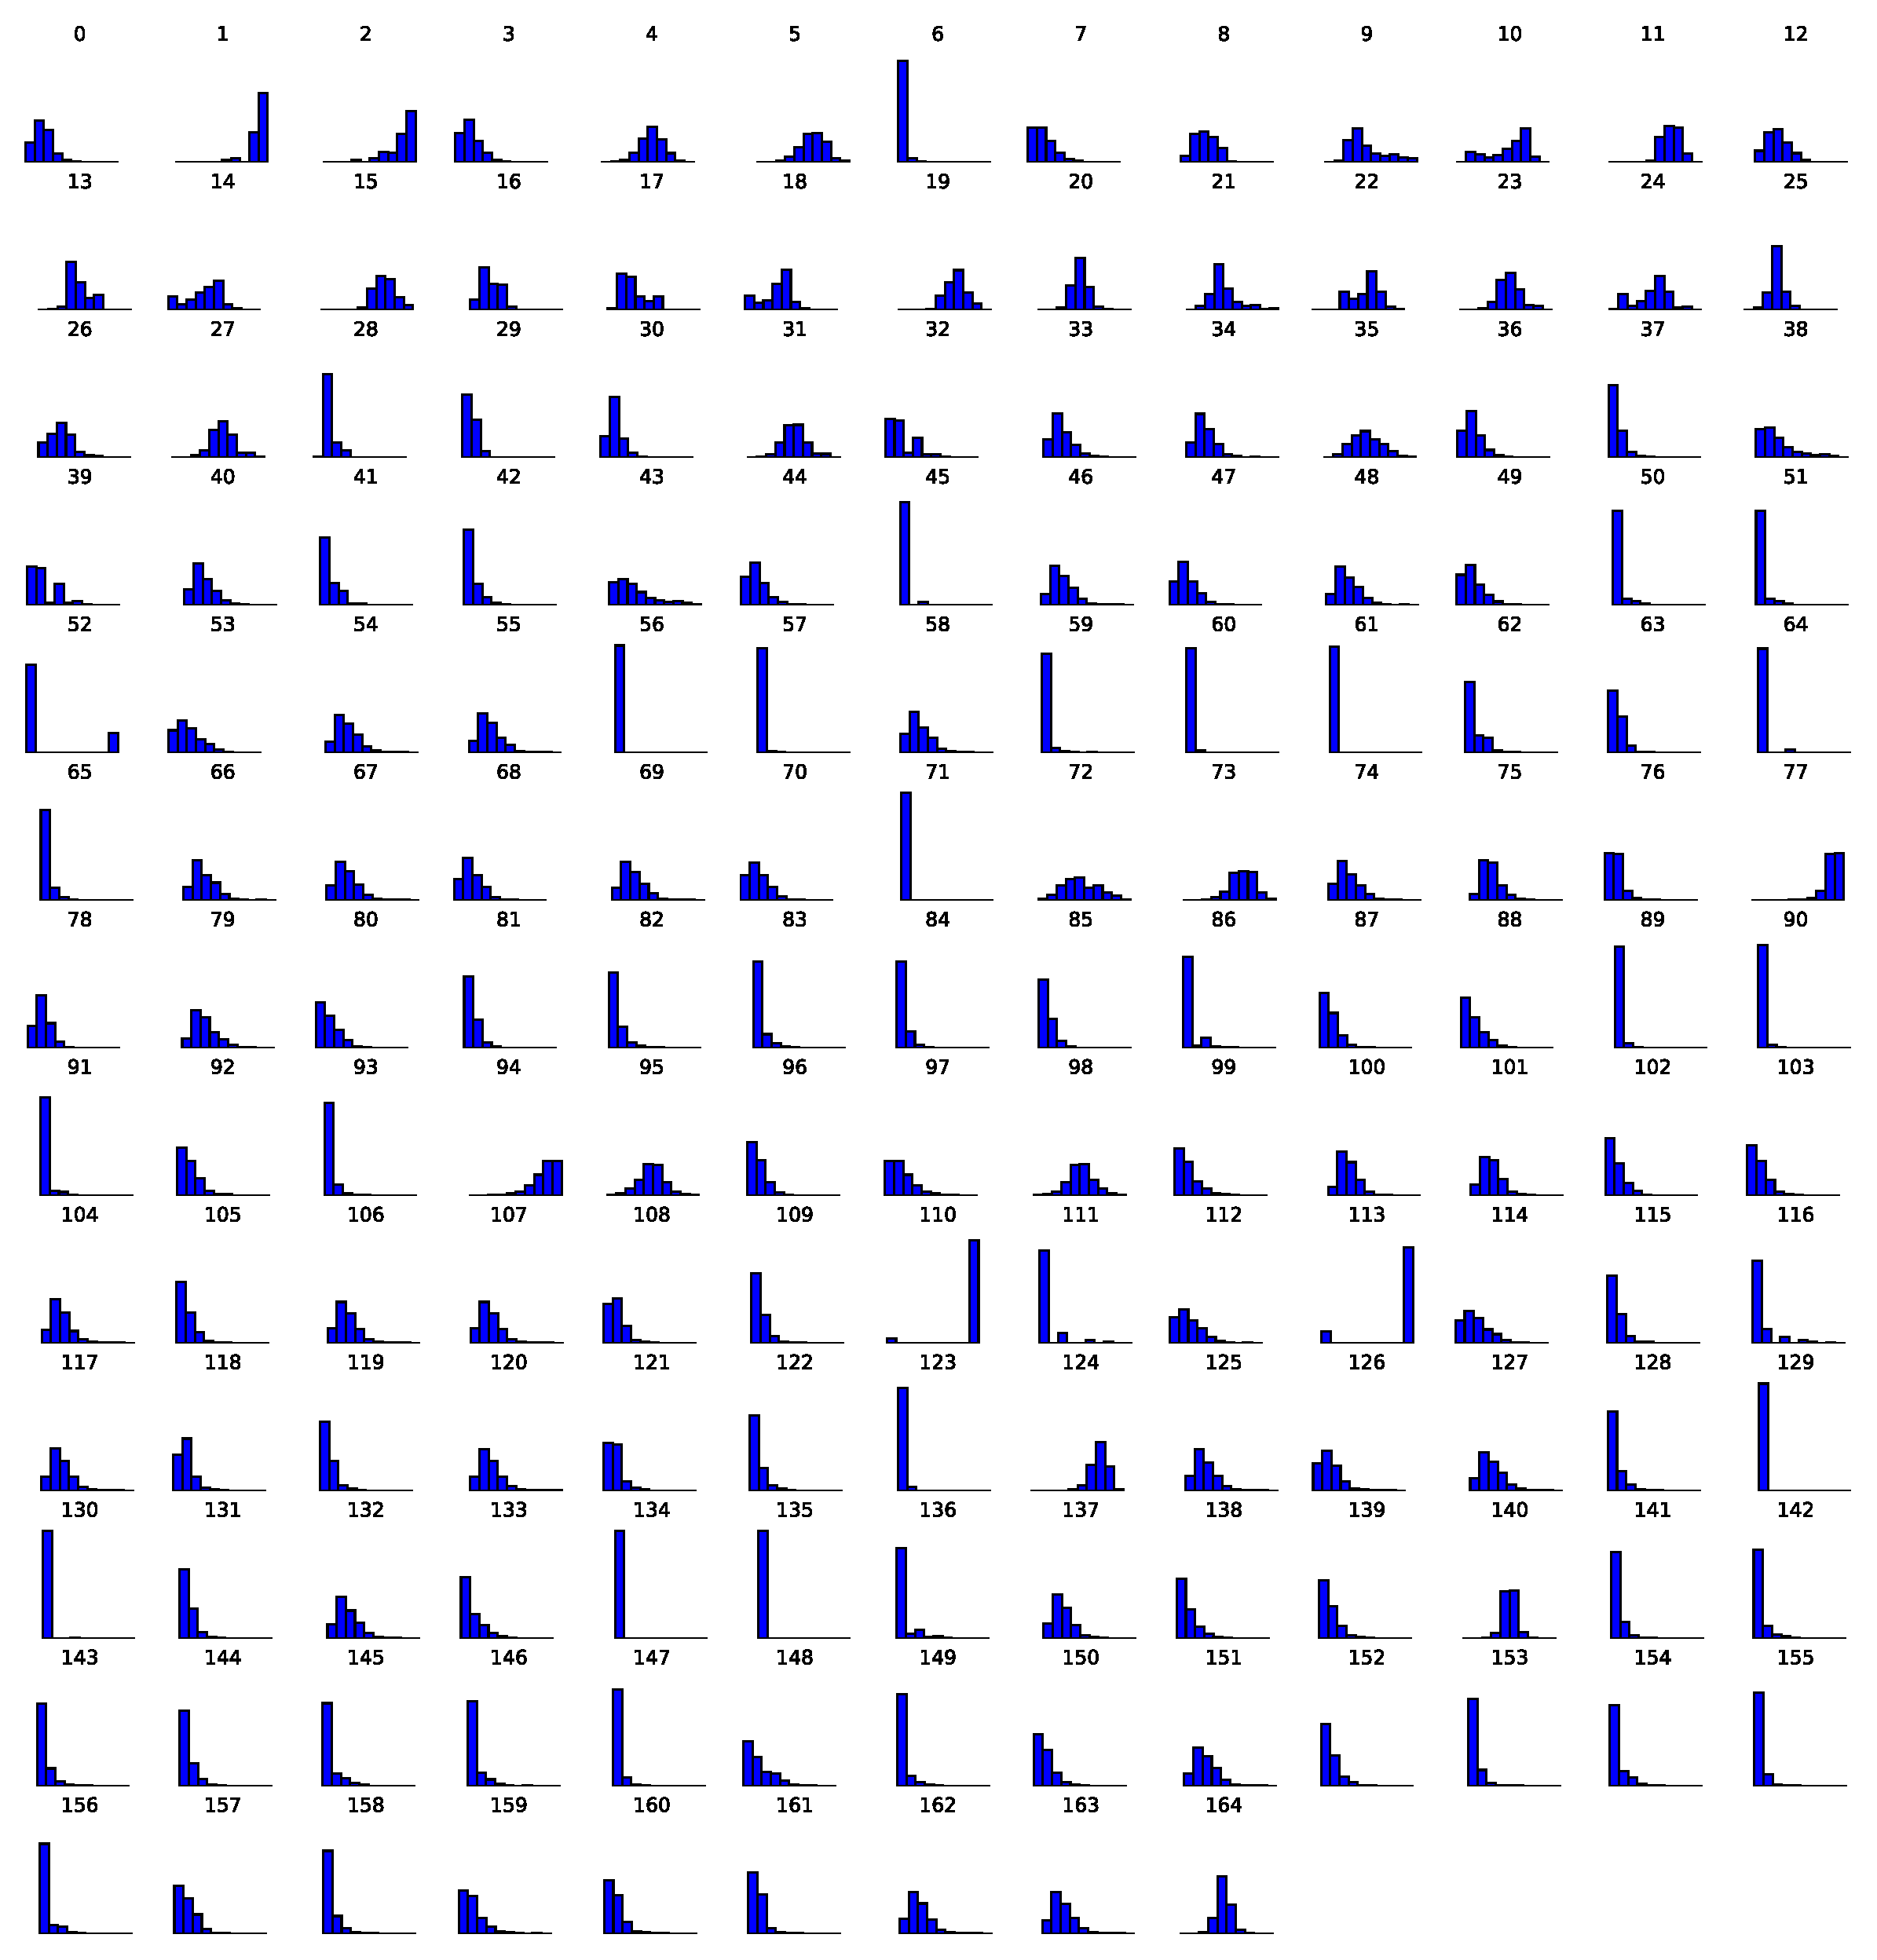
\includegraphics[width=1\textwidth]{RealDataDistr}}
	\caption{Распределение объектов по значениям признаков}
	\label{fg:realFeatures}
\end{figure*}



\begin{table*}[p]%\small
	\caption{Количество связывающихся с рецепторами лигандов}
	\label{t:dataDescr}
	\centering\medskip%\tabcolsep=2pt%\small
	\begin{tabular}{lrrr}
		\headline
		
		Рецептор
		
		& Неизвестно
		& Не связывается
		& Связывается\\
		
		\headline
		{\tt NR-AhR}
		& $\mathbf{3413}\, (40 \%)$
		& $\mathbf{4503}\, (52 \%)$
		& $\mathbf{597}\, (7 \%)$\\
		
		{\tt NR-AR-LBD}
		& $\mathbf{3213}\, (37 \%)$
		& $\mathbf{5129}\, (60 \%)$
		& $\mathbf{171}\, (2 \%)$\\
		
		{\tt NR-AR}
		& $\mathbf{2904}\, (34 \%)$
		& $\mathbf{5398}\, (63 \%)$
		& $\mathbf{211}\, (2 \%)$\\
		
		{\tt SR-MMP}
		& $\mathbf{3925}\, (46 \%)$
		& $\mathbf{3870}\, (45 \%)$
		& $\mathbf{718}\, (8 \%)$\\
		
		{\tt NR-ER}
		& $\mathbf{3746}\, (44 \%)$
		& $\mathbf{4232}\, (49 \%)$
		& $\mathbf{535}\, (6 \%)$\\
		
		{\tt SR-HSE}
		& $\mathbf{3309}\, (38 \%)$
		& $\mathbf{4961}\, (58 \%)$
		& $\mathbf{243}\, (2 \%)$\\
		
		{\tt SR-p53}
		& $\mathbf{3174}\, (37 \%)$
		& $\mathbf{5029}\, (59 \%)$
		& $\mathbf{310}\, (3 \%)$\\
		
		{\tt NR-PPAR-gamma}
		& $\mathbf{3393}\, (39 \%)$
		& $\mathbf{4987}\, (58 \%)$
		& $\mathbf{133}\, (1 \%)$\\
		
		{\tt SR-ARE}
		& $\mathbf{3791}\, (44 \%)$
		& $\mathbf{4029}\, (47 \%)$
		& $\mathbf{693}\, (8 \%)$\\
		
		{\tt NR-Aromatase}
		& $\mathbf{4544}\, (53 \%)$
		& $\mathbf{3835}\, (45 \%)$
		& $\mathbf{134}\, (1 \%)$\\
		
		{\tt SR-ATAD5}
		& $\mathbf{2951}\, (34 \%)$
		& $\mathbf{5360}\, (62 \%)$
		& $\mathbf{202}\, (2 \%)$\\
		
		{\tt NR-ER-LBD}
		& $\mathbf{3107}\, (36 \%)$
		& $\mathbf{5168}\, (60 \%)$
		& $\mathbf{238}\, (2 \%)$\\
		\hline
	\end{tabular}
\end{table*}

\begin{table}[H]%\small
	\caption{Значение AUC для различных рецепторов и моделей классификации}
	\label{t:methodCmp}
	\centering\medskip%\tabcolsep=2pt%\small
	\begin{tabular}{lrr}
		\headline
		
		Рецептор
		
		& Binary Relevance
		& Random Forest \cite{qsar} \\
		
		\headline
		
		{\tt NR-AhR}
		& $\mathbf{0.83} \pm 0.03$
		& $\mathbf{0.93}$ \\
		
		{\tt NR-AR-LBD}
		& $\mathbf{0.86} \pm 0.08$
		& $\mathbf{0.88}$ \\
		
		{\tt NR-AR}
		& $\mathbf{0.83} \pm 0.09$
		& $\mathbf{0.83}$ \\
		
		{\tt SR-MMP}
		& $\mathbf{0.87} \pm 0.03$
		& $\mathbf{0.95}$ \\
		
		{\tt NR-ER}
		& $\mathbf{0.78} \pm 0.04$
		& $\mathbf{0.81}$ \\
		
		{\tt SR-HSE}
		& $\mathbf{0.79} \pm 0.04$
		& $\mathbf{0.86}$ \\
		
		{\tt SR-p53}
		& $\mathbf{0.79} \pm 0.07$
		& $\mathbf{0.88}$ \\
		
		{\tt NR-PPAR-gamma}
		& $\mathbf{0.79} \pm 0.04$
		& $\mathbf{0.86}$ \\
		
		{\tt SR-ARE}
		& $\mathbf{0.78} \pm 0.02$
		& $\mathbf{0.84}$ \\
		
		{\tt NR-Aromatase}
		& $\mathbf{0.81} \pm 0.05$
		& $\mathbf{0.84}$ \\
		
		{\tt SR-ATAD5}
		& $\mathbf{0.81} \pm 0.06$
		& $\mathbf{0.83}$ \\
		
		{\tt NR-ER-LBD}
		& $\mathbf{0.80} \pm 0.07$
		& $\mathbf{0.83}$ \\
		\hline
	\end{tabular}
\end{table}

\begin{figure*}[p]
	\subfloat[Рецептор NR-AhR]{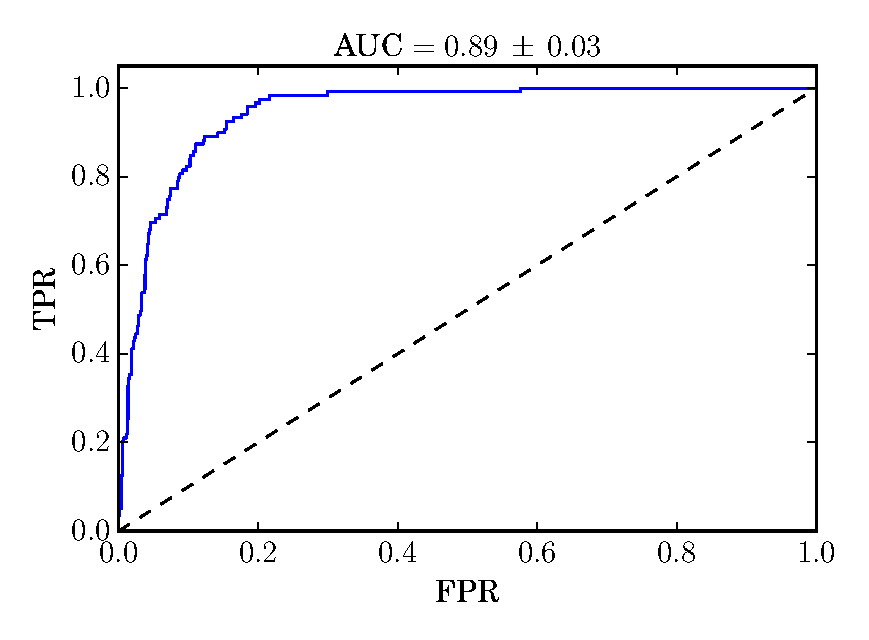
\includegraphics[width=0.3\textwidth]{class1}}
	\subfloat[Рецептор NR-AR-LBD]{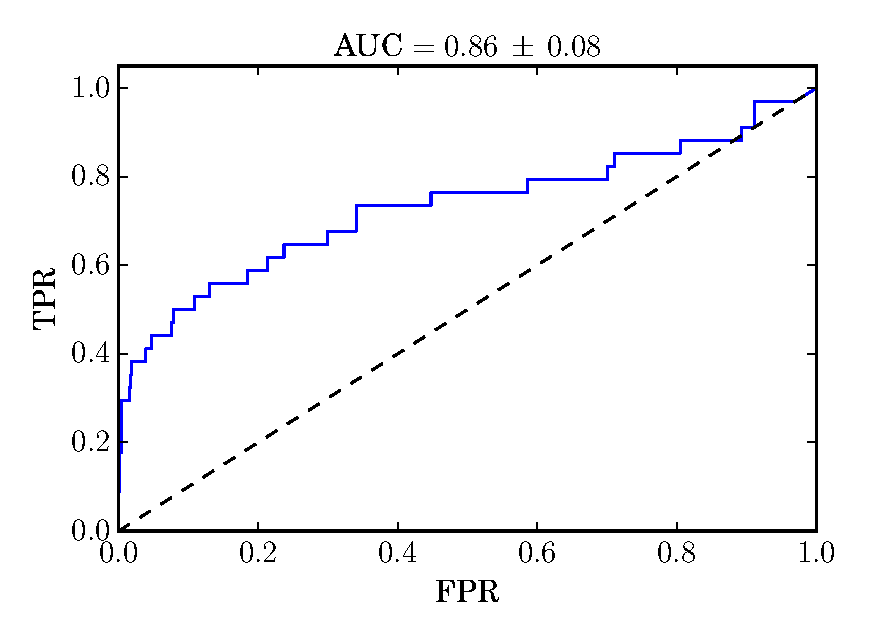
\includegraphics[width=0.3\textwidth]{class2}}
	\subfloat[Рецептор NR-AR]{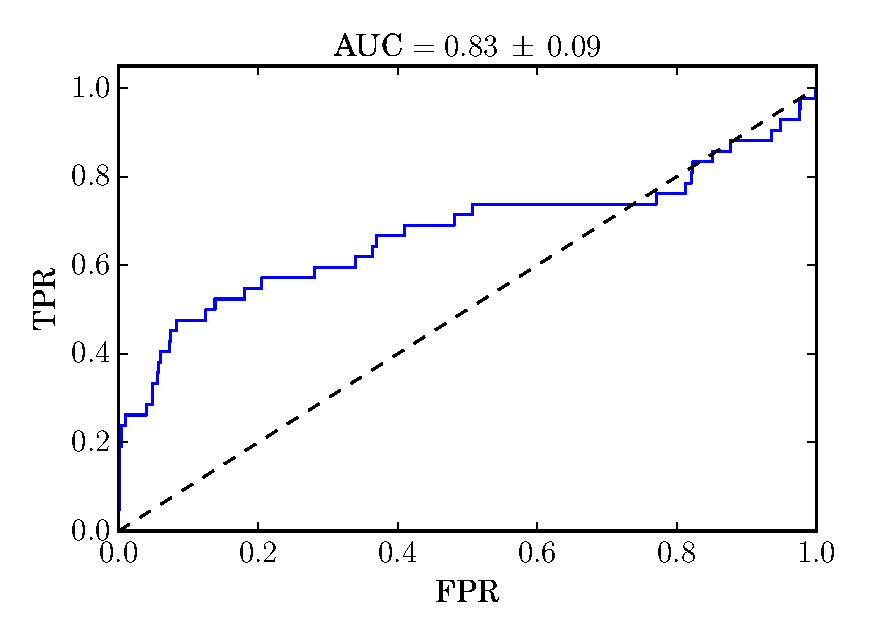
\includegraphics[width=0.3\textwidth]{class3}}\\
	\subfloat[Рецептор SR-MMP]{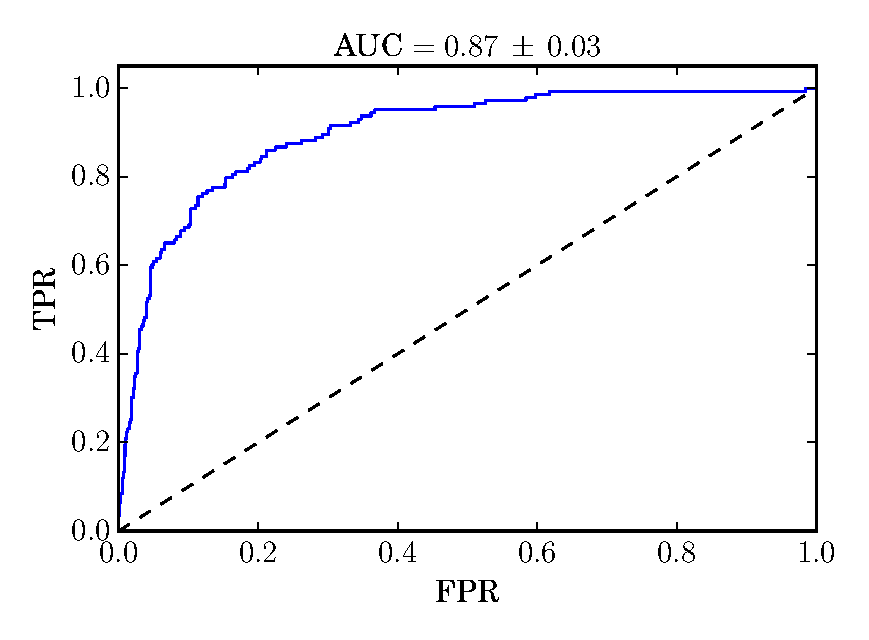
\includegraphics[width=0.3\textwidth]{class4}}
	\subfloat[Рецептор NR-ER]{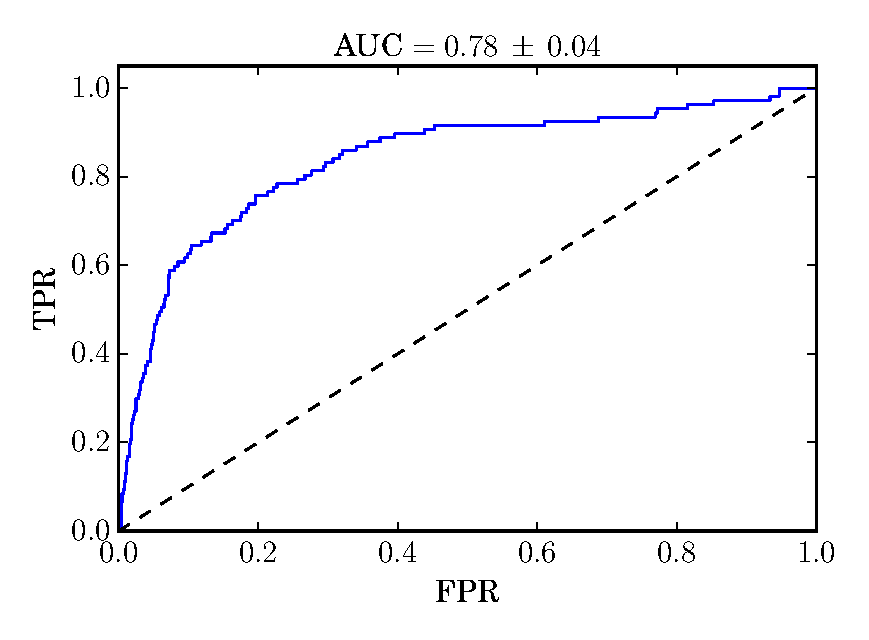
\includegraphics[width=0.3\textwidth]{class5}}
	\subfloat[Рецептор SR-HSE]{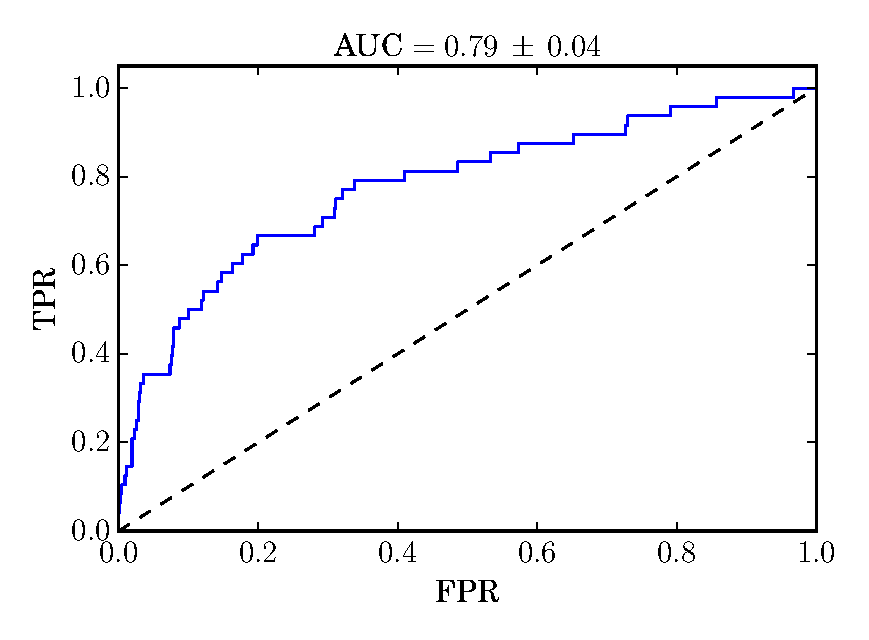
\includegraphics[width=0.3\textwidth]{class6}}\\
	\subfloat[Рецептор SR-p53]{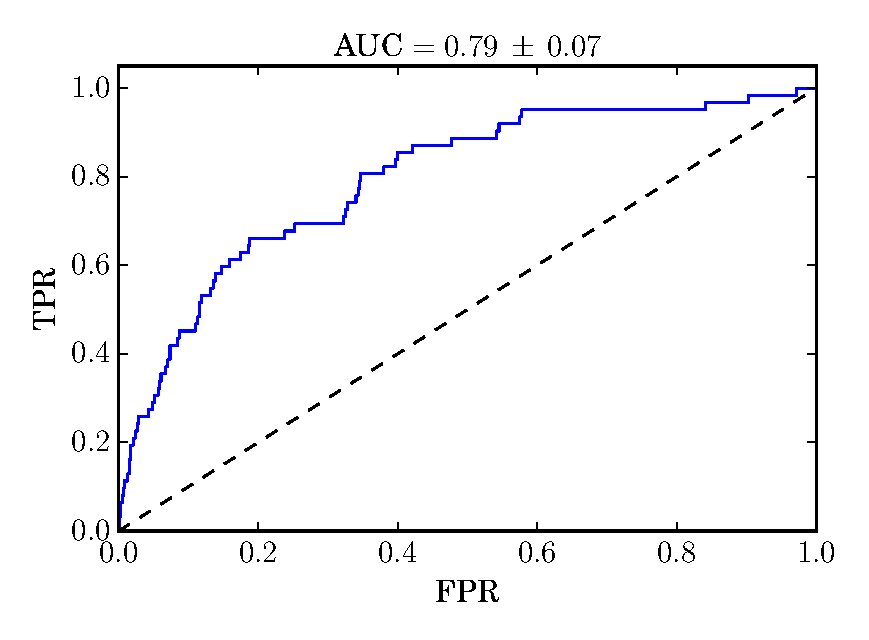
\includegraphics[width=0.3\textwidth]{class7}}
	\subfloat[Рецептор NR-PPAR-gamma]{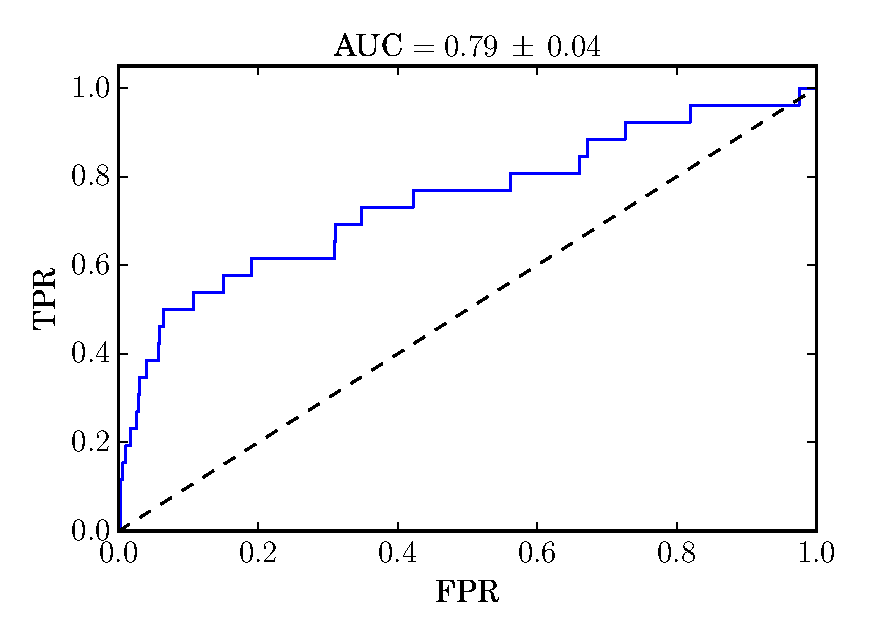
\includegraphics[width=0.3\textwidth]{class8}}
	\subfloat[Рецептор SR-ARE]{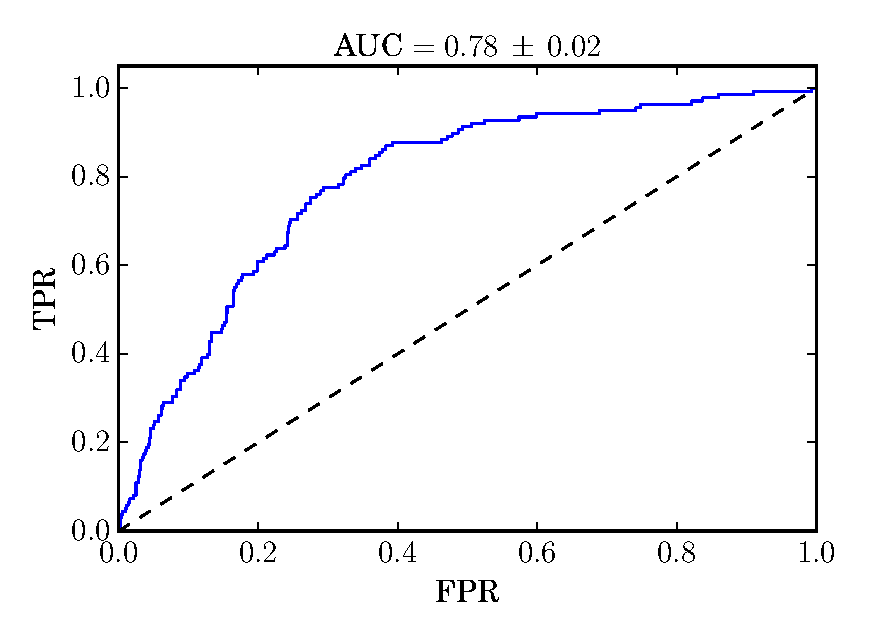
\includegraphics[width=0.3\textwidth]{class9}}\\
	\subfloat[Рецептор NR-Aromatase]{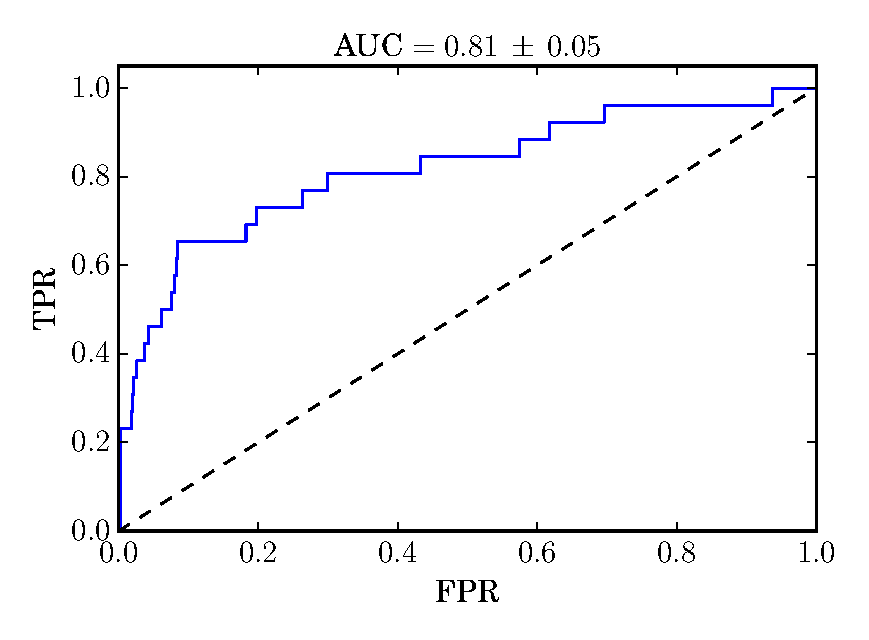
\includegraphics[width=0.3\textwidth]{class10}}
	\subfloat[Рецептор SR-ATAD5]{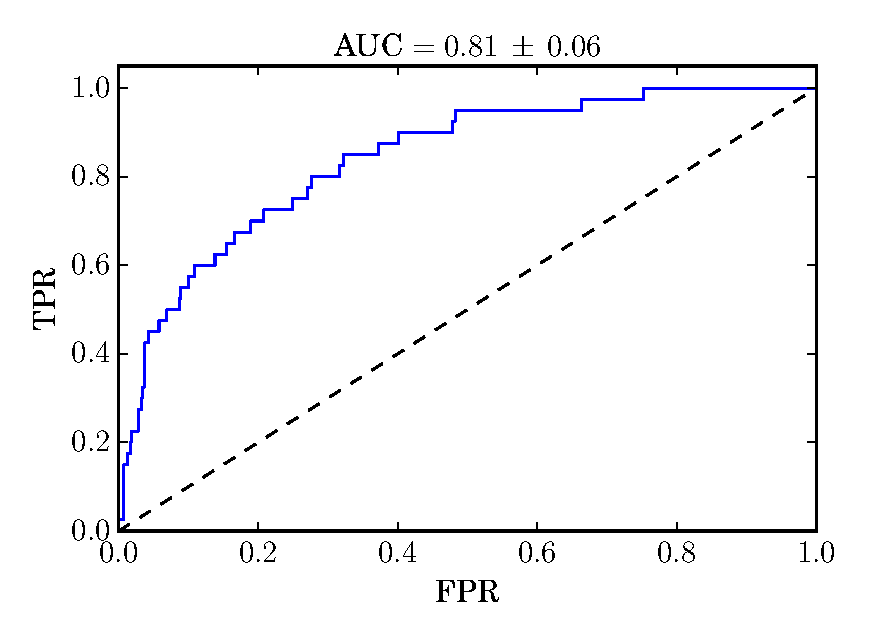
\includegraphics[width=0.3\textwidth]{class11}}
	\subfloat[Рецептор NR-ER-LBD]{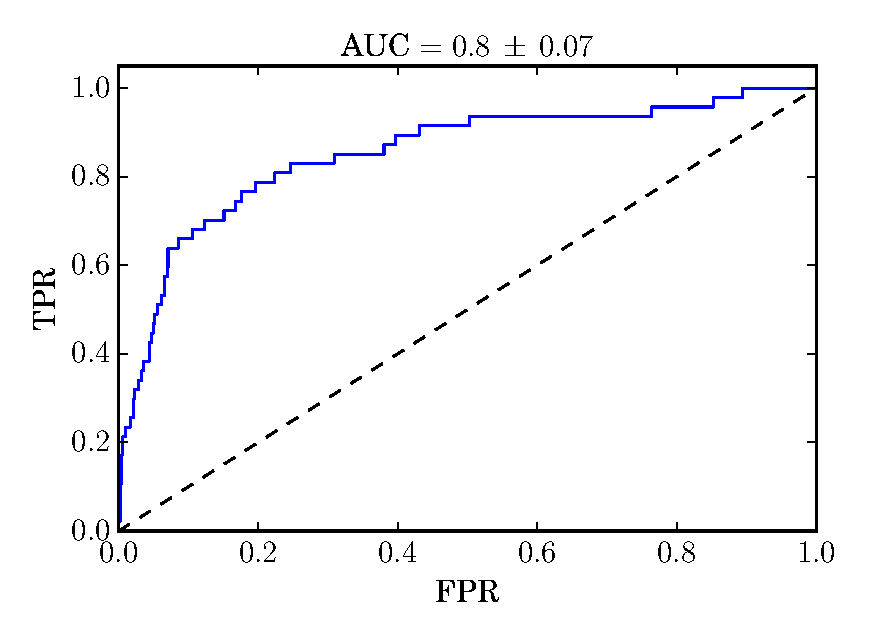
\includegraphics[width=0.3\textwidth]{class12}}\\
	\caption{ROC-кривая и значения функционала AUC для классов 1-12, метод Binary Relevance}
	\label{fg:BR}
\end{figure*}

\begin{table*}[p]%\small
	\caption{Сравнение алгоритмов на модельных данных}
	\label{t:modelData}
	\centering\medskip%\tabcolsep=2pt%\small
	\begin{tabular}{lrrrr}
		\headline
		Метрика &             BR &         PCC (H) &         PCC (M) &         PCC (S) \\
		\headline
		AUC 1 &   0.69 $\pm$ 0.03 &  0.69 $\pm$ 0.03 &  0.69 $\pm$ 0.02 &  0.69 $\pm$ 0.05 \\
		AUC 2 &   0.55 $\pm$ 0.04 &  0.55 $\pm$ 0.04 &  0.56 $\pm$ 0.03 &  0.51 $\pm$ 0.04 \\
		AUC 3 &   0.65 $\pm$ 0.04 &  0.66 $\pm$ 0.02 &  0.64 $\pm$ 0.04 &  0.64 $\pm$ 0.04 \\
		H     &  0.37 $\pm$ 0.009 &  0.36 $\pm$ 0.02 &  0.36 $\pm$ 0.02 &  0.38 $\pm$ 0.04 \\
		H 1   &   0.31 $\pm$ 0.03 &  0.31 $\pm$ 0.03 &  0.31 $\pm$ 0.02 &  0.31 $\pm$ 0.05 \\
		H 2   &   0.45 $\pm$ 0.04 &  0.45 $\pm$ 0.04 &  0.45 $\pm$ 0.03 &  0.49 $\pm$ 0.05 \\
		H 3   &   0.34 $\pm$ 0.03 &   0.3 $\pm$ 0.03 &  0.31 $\pm$ 0.04 &  0.34 $\pm$ 0.03 \\
		P 1   &    0.7 $\pm$ 0.06 &   0.7 $\pm$ 0.06 &  0.73 $\pm$ 0.05 &  0.64 $\pm$ 0.05 \\
		P 2   &   0.55 $\pm$ 0.04 &  0.51 $\pm$ 0.01 &  0.47 $\pm$ 0.04 &  0.46 $\pm$ 0.07 \\
		P 3   &    0.7 $\pm$ 0.06 &  0.56 $\pm$ 0.05 &    0.5 $\pm$ 0.1 &  0.66 $\pm$ 0.05 \\
		R 1   &   0.68 $\pm$ 0.04 &  0.68 $\pm$ 0.04 &  0.68 $\pm$ 0.03 &  0.71 $\pm$ 0.05 \\
		R 2   &    0.52 $\pm$ 0.1 &   0.53 $\pm$ 0.1 &  0.54 $\pm$ 0.09 &  0.48 $\pm$ 0.05 \\
		R 3   &    0.48 $\pm$ 0.1 &  0.53 $\pm$ 0.06 &  0.52 $\pm$ 0.07 &  0.49 $\pm$ 0.09 \\
		S     &   0.78 $\pm$ 0.03 &  0.77 $\pm$ 0.05 &  0.77 $\pm$ 0.05 &  0.62 $\pm$ 0.06 \\
		\headline
	\end{tabular}
\end{table*}

\begin{table*}[p]%\small
	\caption{Сравнение алгоритмов на реальных данных. Рецепторы 1,2,3 = NR-AhR, NR-AR-LBD, NR-Aromatase}
	\label{t:realData}
	\centering\medskip%\tabcolsep=2pt%\small
	\begin{tabular}{lrrrr}
		\headline
		{Метрика} &             BR &           PCC (H) &          PCC (M) &           PCC (S) \\
		\headline
		AUC 1 &   0.58 $\pm$ 0.03 &    0.58 $\pm$ 0.03 &    0.57 $\pm$ 0.02 &    0.58 $\pm$ 0.02 \\
		AUC 2 &   0.61 $\pm$ 0.06 &    0.61 $\pm$ 0.06 &    0.62 $\pm$ 0.06 &    0.61 $\pm$ 0.05 \\
		AUC 3 &   0.55 $\pm$ 0.01 &    0.54 $\pm$ 0.01 &    0.53 $\pm$ 0.01 &    0.54 $\pm$ 0.01 \\
		H     &   0.15 $\pm$ 0.01 &    0.17 $\pm$ 0.01 &    0.19 $\pm$ 0.02 &    0.17 $\pm$ 0.02 \\
		H 1   &   0.21 $\pm$ 0.03 &    0.21 $\pm$ 0.03 &    0.24 $\pm$ 0.02 &    0.21 $\pm$ 0.03 \\
		H 2   &  0.045 $\pm$ 0.01 &  0.041 $\pm$ 0.007 &  0.041 $\pm$ 0.008 &  0.041 $\pm$ 0.006 \\
		H 3   &    0.2 $\pm$ 0.02 &    0.25 $\pm$ 0.01 &    0.29 $\pm$ 0.03 &    0.25 $\pm$ 0.03 \\
		P 1   &    0.79 $\pm$ 0.1 &     0.79 $\pm$ 0.1 &     0.79 $\pm$ 0.1 &     0.82 $\pm$ 0.1 \\
		P 2   &    0.91 $\pm$ 0.1 &     0.88 $\pm$ 0.1 &     0.91 $\pm$ 0.1 &     0.88 $\pm$ 0.1 \\
		P 3   &   0.76 $\pm$ 0.07 &    0.82 $\pm$ 0.09 &    0.78 $\pm$ 0.09 &    0.82 $\pm$ 0.08 \\
		R 1   &   0.17 $\pm$ 0.06 &    0.17 $\pm$ 0.06 &    0.15 $\pm$ 0.04 &    0.18 $\pm$ 0.05 \\
		R 2   &    0.22 $\pm$ 0.1 &     0.23 $\pm$ 0.1 &     0.24 $\pm$ 0.1 &     0.23 $\pm$ 0.1 \\
		R 3   &    0.1 $\pm$ 0.02 &   0.085 $\pm$ 0.02 &   0.071 $\pm$ 0.02 &   0.086 $\pm$ 0.02 \\
		S     &   0.32 $\pm$ 0.02 &    0.34 $\pm$ 0.02 &    0.46 $\pm$ 0.03 &     0.3 $\pm$ 0.03 \\
		\headline
	\end{tabular}
\end{table*}

\bibliographystyle{unsrt}
\clearpage
\bibliography{Volodin2016ProbabilisticReceptorPrediction}
% Решение Программного Комитета:
%\ACCEPTNOTE
%\AMENDNOTE
%\REJECTNOTE
\end{document}
